\documentclass[main]{subfiles}
\begin{document}
\section{Teori}
%\subsection{Diffraktion  af lysbølge}
%Når en bølge af lys eller lyd propagerer igennem snævre åbninger på størrelse med bølgelængden, vil bølgen spredes i mønstre bestemt ud fra bølgeegenskaber som destruktiv og konstruktiv interferens. Dette bølgefænomen kaldes diffraktion, og er grundlæggende for denne rapport. Ved
%

\subsection{Akusto-Optisk Modulator}
En akusto-optisk modulator (AOM) er en brugbar komponent til modulation af frekvens, intensitet og retning af en laser stråle. Den består af en Piezo Elektrish Transducer (PZT), en gennemsigtig krystal og en akustisk absorber. Fra PZT'en genereres mekaniske vibrationer som propagerer longitudinelt op gennem krystallen. Denne bølge er en lydbølge (deraf akustisk), og kan derfor betragtes som en variation af tætheder. Ved tæthedstoppe er brydningsindekset maksimalt, og ved tæthedsdale er den minimal. Når lys stråler ind på en sådan gradient af brydningsindices vil det spredes.

Lys fra følgende akustiske bølgefronte vil interferere konstruktivt. Lydbølgen fungerer som et almindeligt diffraktionsgitter for den indkommende laser og der dannes et diffraktionsmønster.
Kravet for konstruktiv interferens af laseren er
\begin{equation}
    n\lambda_L = \lambda_S \left( \sin\theta_i + \sin\theta_d \right)
    \label{reduktion}
\end{equation}
hvor indekserne $L$ og $S$ er for respektivt \emph{light} og \emph{sound}. Her er $n=1,2,\cdots$ et heltal som angiver hvilken orden der er tale om. De to vinkler $\theta_i$ og $\theta_d$ er indfalds- og udfaldsvinklen for lyset, når det interagerer med den akustiske bølgefront.

For optiske bølger med en frekvens af størrelsesorden $10^8\si{\hertz}$ kan det vises\footnote{\url{http://massey.dur.ac.uk/resources/slcornish/AOMGuide.pdf}} fra energi- og impulsbevarlse, at $\theta_i = \theta_d$, hvorfor \cref{reduktion} kan reduceres til
\begin{equation}
    n\lambda_L = 2\lambda_S \sin(\theta_d)
    \label{eq:interferens}
\end{equation}
%\begin{equation}
%    n(x,t) = n_0 + \Delta n \cos(k_s x - \omega t).
%    \label{eq:brydningsindeks}
%\end{equation}
%Resultatet af en lydbølge i et transparent medie er denne tæthedsfunktion, hvor $n_0$ er den uforstyrret brydningsindekset, $\omega$ er vinkelfrekvensen, $k=\frac{2\pi}{\lambda}$ er bølgetallet for lydbølgen og $\Delta n$ er variationen af amplituden i det brydningsindekset, genereret af lydbølgen.
%
%Det er denne rejsende variation i krystallets tæthed, som skal fungere som diffraktionsgitter for den indkommende laser. Sidstnævnte absorber har til formål at absorbere størstedelen af lydbølgen, så der ikke vil reflekteres energi tilbage i krystallen.
%
%Den genererede brydningsindeks giver anledning til et diffraktionsgitter som rejser med lydens hastighed i krystallet som medie. Lys som propagerer igennem det transparente materiale vil diffraktere grundet denne genererede brydningsindeks. Derfor forventes et diffraktionsmønster såfremt man stiller en skærm i en vis afstand fra AOM'en.
%
%Her gælder de konventionele formler for konstruktiv interferens ved vinkler
%\begin{equation}
%    d\sin\theta_m = m\lambda,
%    \label{eq:konstruktiv}
%\end{equation}
%
%\begin{equation}
%    f_n = f_0 \pm nf_s, \qquad n=0, \pm1, \pm2, \cdots
%    \label{eq:frequence}
%\end{equation}
%hvor $f_0$ er den upåvirkede frekvens, $f_s$ er lydens frekvens og $n$ er den valgte orden.
\subsection{Regimer}
Når lys diffrakteres af en lydbølge med en enkelt frekvens, vil der være to diffraktionstyper. Raman-Nath og Bragg Diffraktion.

Raman-Nath diffraktion observeres ved lave lydfrekvenser (omkring $\SI{10}{\mega\hertz}$ og smal længde $L$ for den akusto-optiske interaktioner (bredden af krystallen). Denne type sker for vilkårlige indfaldsvinkler.
Bragg diffraktion vil modsat være ved høj lydfrekvens (omkring $\SI{100}{\mega\hertz}$). For Bragg diffraktion vil der primært være to diffraktions maksima; nulte og første orden.

For at skelne de to regimer bruges betingelsesværdien for Bragg og Raman-Nath af $Q>>1$ og $Q<<1$ respektivt. $Q$ kaldes her for Klein-Cook parameteren og er givet ved
\begin{equation}
    Q = \frac{2\pi\lambda_L L {f_{S}}^2}{n{v}_{S}^2}=\frac{2\pi\lambda_L L}{n{\lambda_S}^2}
\label{eq:KleinCook}
\end{equation}
Her er $L$ interaktionslængden mellem den akustiske og optiske bølge.

I forsøget vil der være primært interesse i første orden $n=1$, hvorfor Bragg-regimet er ønsket, da der her er mindst effekt-tab i laserstrålen. Bragg-diffraktion præger dog forsøget med sine betingelser for lydfrekvensen og dermed også lydens hastighed.

Når lyset spredes gælder det, at vinklen mellem nulte og første orden er givet ved
\begin{equation}
    \theta_{sep} = 2 \theta_B = \frac{\lambda_L f_S}{v_S},
    \label{eq:sep}
\end{equation}
hvor $\theta_B$ er Bragg vinklen.

En anden måde at tolke denne interaktion mellem lyd og lys er ved at betragte det som et stød mellem begges partikelmodel. Fotonens impuls ændres idet fononen støder ind i den, og dens energi overføres til fotonen. Det vil der dog ikke gøres mere ud af i denne rapport.

\subsection{Effektivitet}
I forsøget vil forholdet mellem lydbølgernes amplitude og laserens intensitet undersøges. Der gælder at intensiteten for $n=1$ er
\begin{equation}
    I_1 = I_0 \sin^2\left(\sqrt{\eta}\right)
    \label{eq:Intensitet}
\end{equation}
hvor $\eta = \frac{\pi^2}{4}\frac{P_1}{P_0}$, og $P_0 = \frac{\lambda^2}{2 n_2}\frac{H}{L}$. Her er $P$ effekten af laserstrålen i hhv. nulte og første orden, og desuden introduceres $n_2$ nu som den akusto-optiske koefficient. Den sidste brøk er ren geometrisk, hvor $H$ er højden af lydbølgen, og $L$ er den førnævnte interaktions længde (krystallens længde).

Når det plotts, kan det forventes et peak ved en bestemt $P=P_0$.

\subsection{Gaussisk Stråle}
Fra geometrisk optik vil lys fokuseres til et punkt ved at propagerere gennem en konkav linse. Dette punkt kaldes fokalpunktet.
Der vil nu bruges en anden model, som beskrive dette punkt som en minimal afstand, og ikke et samlepunkt. Den minimale afstand kaldes for strålens \emph{waist} og betegnes $w_0$.

I forsøget bruges til en god approksimation en monokromatisk laserstråle. Den kan tilnærme sig en Gaussisk stråle, da dens tranversale magnetiske-- og elektriske feltbølgers amplitude kan beskrives ved en Gauss funktion. Den fundamentale tranversale gaussiske tilstand ($TEM_{00}$) beskriver mange lasere\footnote{\url{https://en.wikipedia.org/wiki/Gaussian_beam}}. For en given bølgelængde $\lambda$ beskrives en gaussisk stråle af én parameter $w_0$ kaldet laserens \emph{waist}. Strålens waist er et mål for strålens størrelse ved fokalpunktet ($z=0$). Her er strålens bredde minimal, og intensiteten er størst. Bredden er en funktion af $z$, hvor $z$ er afstanden relativt til fokalpunktet.

\subsection{Hastighed for switch af lys}
Så længe lydbølgen opretholdes af PZT'en, vil der være diffraktion. Vil man måle hastigheden for at tænde / slukke for lyset, kan man slukke for PZT'en. Dette er vist på \cref{fig:risefall}.  I det lyden tøver vil der være en responstid fra at lyden slukkes til sidste bølgetop passerer target, og denne tid må være proportional med lydens hastighed samt targets størrelse.
\begin{equation}
    T_R \propto \frac{A}{v_S}.
\end{equation}
Hvor $T_R$ er defineret til at være tiden der tager intensiteten til at gå fra $ 10\% - 90\%$.  Hertil bruges
\begin{align}
    T_R & = T_{90\%} - T_{10\%} = 0.64 \frac{2w_0}{v_S}.\label{eq:risetime} \\
    \Rightarrow v_S & = 0.64 \frac{2w_0}{T_R}.    \label{eq:risetimeIsolere}
\end{align}
\begin{figure}[H]
    \centering
    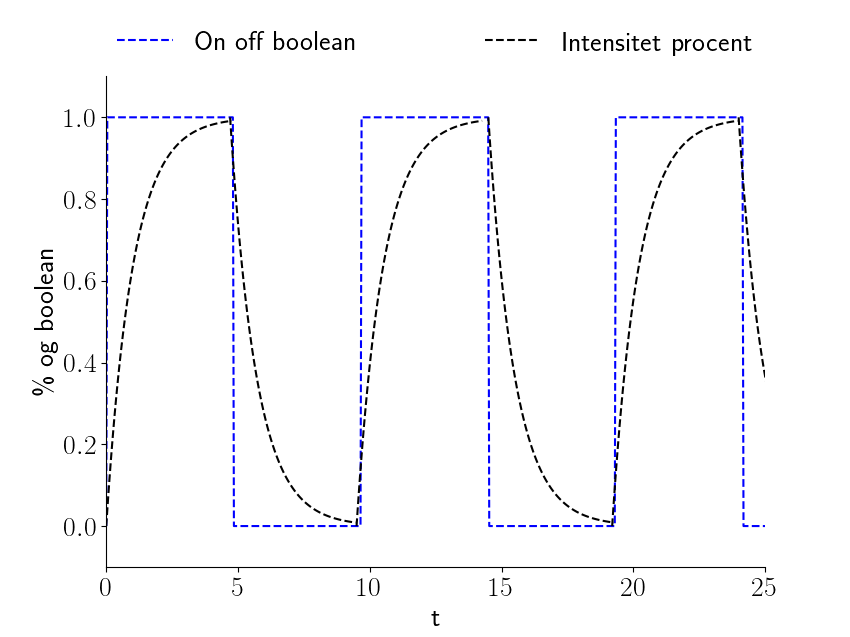
\includegraphics[width=\linewidth]{tegninger/risefall.png}
    \caption{Rise/fall af intensiteten, når swithcen tænder og slukker. }
    \label{fig:risefall}
\end{figure}
\subsection{Intensitet ved hjælp af errorfunction}
I databehandlingen vil det have interesse at bestemme strålens waist, $w_0$, og hertil fittes til følgende formel
\begin{equation}
    I(z) = \text{erf}\left( \frac{x\sqrt{2}}{w_0} \right)
    \label{eq:errorfunc}
\end{equation}

\end{document}
